\documentclass[10pt,a4paper,twocolumn]{article}
\usepackage[utf8]{inputenc}
\usepackage[T1]{fontenc}
\usepackage[english]{babel}
\usepackage[margin=1.8cm,top=2cm,bottom=2cm]{geometry}
\usepackage{graphicx}
\usepackage{booktabs}
\usepackage{amsmath}
\usepackage{listings}
\usepackage{xcolor}
\usepackage{hyperref}
\usepackage{enumitem}
\usepackage{caption}
\usepackage{subcaption}
\usepackage{colortbl}

\setlength{\columnsep}{0.6cm}
\setlist{noitemsep,topsep=2pt}
\captionsetup{font=small,labelfont=bf}

\lstset{
  basicstyle=\ttfamily\scriptsize,
  keywordstyle=\color{blue!70!black},
  commentstyle=\color{green!50!black},
  breaklines=true,
  frame=single,
  xleftmargin=2mm,
  framexleftmargin=2mm,
  columns=fullflexible,
}

\title{\vspace{-1.5em}\textbf{SPM Module 2: Partitioned Hash Join with Duplicates}\vspace{-0.5em}}
\author{Gabriele Marsili}
\date{}

\begin{document}
\maketitle
\vspace{-1.5em}

% ===========================================================================
\section{Parallelization Strategy}
% ===========================================================================

The partitioned hash join pipeline consists of five phases: \textit{Histogram}, \textit{Prefix Sum}, \textit{Scatter}, \textit{Join Local}, and a final sequential \textit{Accumulation}. Each phase has distinct computational and memory characteristics that determine whether parallelism is beneficial and which strategy to adopt.

\subsection*{Thread Team and Barrier Synchronization}

A single team of $k$ threads is launched once and reused across all phases via \texttt{std::barrier} (C++20). An alternative design would use a thread pool with a task queue, but it would introduce unnecessary indirection: because all threads must finish each phase before the next one can begin --- due to data dependencies between histogram, prefix sum, scatter, and join --- a full barrier is required at every phase boundary regardless. The barrier approach directly models this bulk-synchronous structure and avoids the overhead of thread pool bookkeeping (task submission, queue polling, wakeup latency). Spawning and joining threads at each phase boundary would inflate the sequential component $f$ in Amdahl's model by $O(k)$ spawn/join cycles per phase. The barrier completion function runs a single delegate thread between phases to perform the sequential prefix sum and to compute per-thread scatter offsets from the local histograms.

\textbf{Adaptive thread count.} To prevent synchronisation overhead from dominating small workloads, the actual thread count $k$ is:
\[
  k = \min\!\left(k_{\max},\;\left\lfloor \min(NR, NS) \,/\, T_{\min} \right\rfloor\right)
\]
where $k_{\max}$ is the user-requested count and $T_{\min} = 8\,192$ records is the minimum per-thread work threshold. Below this threshold, the cost of barrier synchronisation and cache-line traffic between threads exceeds the parallelism gain. For $NR = 10^7$ and $k_{\max} = 20$ the formula gives $k = \min(20, 1220) = 20$; for $NR = 10^4$ it gives $k = \min(20, 1) = 1$, falling back to a single-threaded execution with no synchronisation overhead.

\subsection*{Histogram (Phases 0 and 2)}

Each thread processes a contiguous block of $\lceil N/k \rceil$ records from relation $R$ (or $S$), incrementing its own private histogram of size $P$. Thread-local histograms eliminate all write contention. After the barrier, the completion delegate merges the $k$ local histograms into a global one in $O(P \cdot k)$ time, then runs the prefix sum $O(P)$ and computes per-thread scatter offsets.

Static block distribution yields good spatial locality: each thread reads a contiguous slice of the input array, maximising cache line utilisation. The dominant cost of this phase is a sequential scan of $N \times 8$\,B of input --- a purely memory-bandwidth-bound operation with very low arithmetic intensity ($I \approx 0.125$\,FLOP/byte). As a consequence, the histogram phase scales poorly with thread count (Section~\ref{sec:results}).

\subsection*{Prefix Sum}

The prefix sum over the $P$-element global histogram is performed sequentially by the barrier completion delegate. With $P \leq 1024$ this takes at most a few microseconds and represents a negligible fraction of total time ($< 0.1\%$ in all measurements). The theoretical span of a parallel prefix sum is $O(\log P)$, but the overhead of synchronising threads for such a small workload would dwarf any gain.

\subsection*{Scatter (Phases 1 and 3)}

Scatter rearranges records into partition-contiguous output arrays. The key property enabling lock-free parallelism is that the per-thread scatter offsets are computed during the barrier: thread $t$ starts writing partition $p$ at offset
\[
  \text{off}[t][p] = \text{global\_begin}[p] + \sum_{j=0}^{t-1} \text{local\_hist}[j][p].
\]
Each thread thus writes to a non-overlapping, pre-determined region of the output array with no synchronisation needed at runtime:

\noindent\begin{minipage}{\linewidth}
\begin{lstlisting}[language=C++]
auto cursor = offsets_R[t]; // local copy on stack
for (size_t i = r_start; i < r_end; ++i) {
    uint32_t pid = hash_key(R[i].key, shift);
    out_R[cursor[pid]++] = R[i];
}
\end{lstlisting}
\end{minipage}

Scatter is memory-bound (random writes driven by hash values), but the absence of any contention allows good parallel throughput. Partition assignment uses the Fibonacci multiply-shift hash from Module~1 (\texttt{hash\_key}: $h(k)=((k_\text{lo}\oplus k_\text{hi})\cdot A_{32})\mathop{>>}s$, $A_{32}=\lfloor 2^{32}/\varphi\rfloor$) rather than the reference $k\bmod P$, giving uniform partition sizes even for structured key sets.

\subsection*{Join Local (Phase 4)}

Each partition can be joined independently: a flat open-addressing hash table \texttt{FlatCountMap} is built on the $R$ slice, then the $S$ slice is probed. This is an embarrassingly parallel workload. Partitions are distributed cyclically: thread $t$ owns partitions $t,\,t{+}k,\,t{+}2k,\ldots$ — zero scheduling overhead, no atomics.

\noindent\begin{minipage}{\linewidth}
\begin{lstlisting}[language=C++,belowskip=0pt,aboveskip=3pt]
for (uint32_t pid = t; pid < P; pid += nt) {
    size_t rb = global_begin_R[pid],
           re = rb + global_hist_R[pid];
    size_t sb = global_begin_S[pid],
           se = sb + global_hist_S[pid];
    if (rb == re || sb == se) continue;
    FlatCountMap countR(re - rb);
    for (size_t i = rb; i < re; ++i)
        countR.increment(out_R[i].key);
    for (size_t i = sb; i < se; ++i) {
        uint32_t m = countR.count(out_S[i].key);
        if (m) { local.join_count += m; ... }
    }
}
\end{lstlisting}
\end{minipage}

For the Fibonacci partitioning hash, partition sizes are statistically near-equal, so cyclic assignment achieves the same load balance as LPT scheduling with zero per-partition synchronisation. Per-thread result accumulators are padded to 64 bytes (\texttt{alignas(64)}) to prevent false sharing. After the barrier, the main thread reduces the partial results.

\subsection*{Summary}

\begin{center}
\small
\begin{tabular}{@{}lll@{}}
\toprule
Phase & Strategy & Bottleneck \\
\midrule
Histogram   & Thread-local + merge & Memory BW \\
Prefix Sum  & Sequential           & Negligible \\
Scatter     & Lock-free offsets    & Memory BW \\
Join Local  & Cyclic distribution  & Compute \\
Accumulate  & Sequential           & Negligible \\
\bottomrule
\end{tabular}
\end{center}

% ===========================================================================
\section{Correctness Verification}
% ===========================================================================

Correctness is verified at two levels. For small inputs ($NR \leq 500$, $NS \leq 500$), both the sequential and parallel binaries automatically run a naive $O(N^2)$ reference join and compare \texttt{join\_count}, \texttt{checksum1}, and \texttt{checksum2}:

\begin{lstlisting}
./hashjoin_par -nr 50 -ns 80 -seed 13 \
  -max-key 8 -p 4 -t 4
# output: naive_verify=PASS
\end{lstlisting}

For large inputs, the same three output values produced by the sequential and parallel binaries are compared across all tested thread counts. Since \texttt{checksum1} and \texttt{checksum2} use independent hash multipliers, the probability of a false positive is negligible. The verification is outside the measured region and does not affect reported timings.

% ===========================================================================
\section{Performance Results}
\label{sec:results}
% ===========================================================================

All experiments were run on a node of the \texttt{spmcluster}: Intel Xeon E5-2640 v2 @ 2.00\,GHz, 2 sockets $\times$ 8 physical cores (16 physical, 32 with Hyper-Threading), NUMA architecture. Default parameters: \texttt{seed=42}, \texttt{max\_key=1M}, \texttt{P=128}, best of 3 repetitions (no CPU pinning; run-to-run variation $\leq 3\%$).

\subsection*{Strong Scaling}

\begin{center}
\small
\begin{tabular}{@{}rrrrrr@{}}
\toprule
$p$ & \multicolumn{2}{c}{NR=10M} & & \multicolumn{2}{c}{NR=20M} \\
\cmidrule{2-3}\cmidrule{5-6}
 & $S(p)$ & $E(p)$ & & $S(p)$ & $E(p)$ \\
\midrule
seq & 1.00 & 100\% & & 1.00 & 100\% \\
1   & 1.04 & 104\% & & 1.02 & 102\% \\
2   & 1.44 &  72\% & & 1.43 &  72\% \\
4   & 2.62 &  66\% & & 2.52 &  63\% \\
8   & 4.57 &  57\% & & 4.43 &  55\% \\
10  & 5.37 &  54\% & & 5.39 &  54\% \\
14  & 6.67 &  48\% & & 6.81 &  49\% \\
\rowcolor{gray!15}
20  & 7.12 &  36\% & & 7.53 &  38\% \\
\rowcolor{gray!15}
24  & 7.99 &  33\% & & 8.56 &  36\% \\
\rowcolor{gray!15}
32  & 8.29 &  26\% & & 9.27 &  29\% \\
\bottomrule
\end{tabular}
\end{center}
{\footnotesize $S(1)>1.0$: the sequential binary stores partitioned data in a \texttt{PartitionedRelation} struct accessed via \texttt{begin}/\texttt{end} vector indirections, whereas the parallel binary (even at $p=1$) uses flat \texttt{global\_begin\_R}/\texttt{global\_hist\_R} arrays with direct index arithmetic. The different memory layouts produce slightly different cache-access patterns, contributing to the 4\% gap (752\,ms vs.\ 782\,ms); without CPU pinning the gap falls within typical run-to-run variation.}

\begin{figure*}[t]
  \centering
  \begin{subfigure}[b]{0.49\textwidth}
    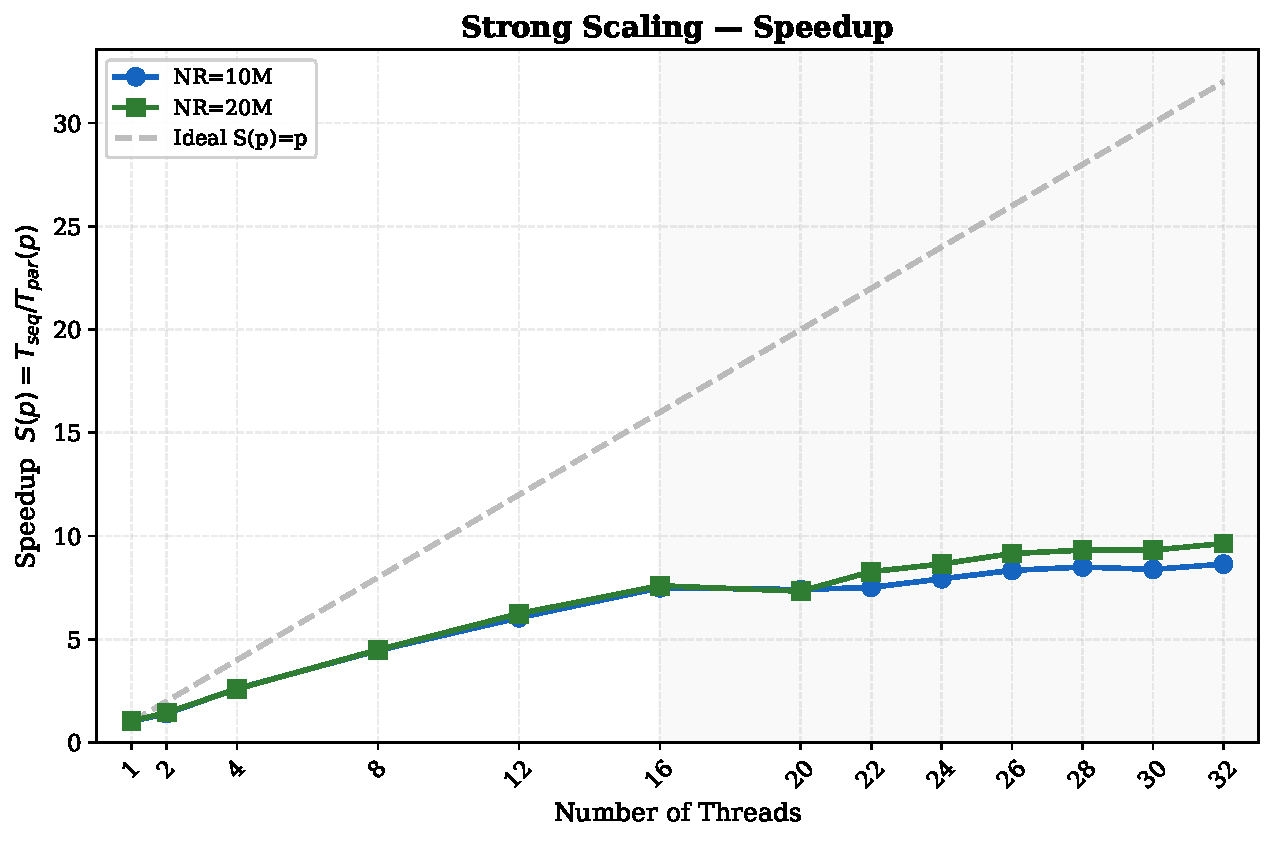
\includegraphics[width=\linewidth]{../results/plots/strong_speedup.pdf}
    \caption{Speedup $S(p) = T_\text{seq}/T_\text{par}(p)$.}
    \label{fig:strong_speedup}
  \end{subfigure}
  \hfill
  \begin{subfigure}[b]{0.49\textwidth}
    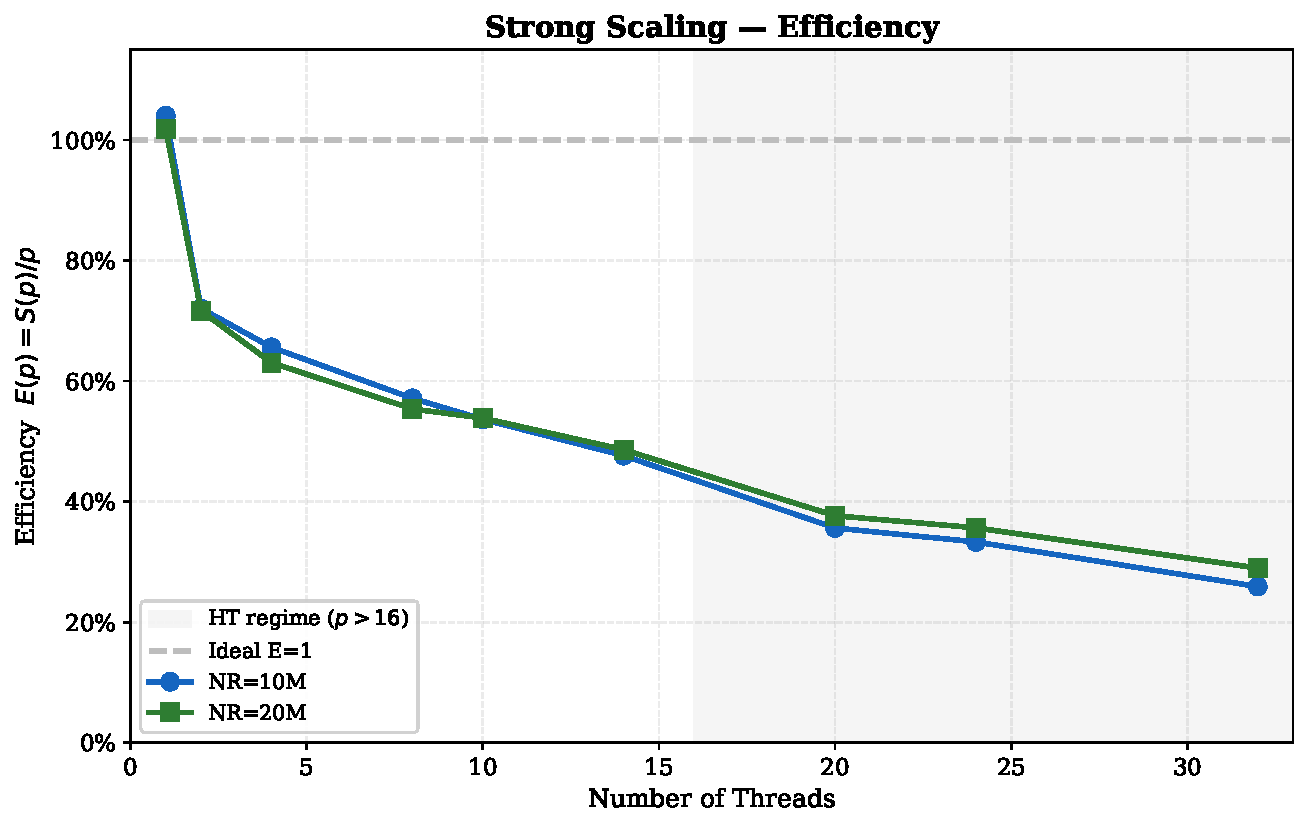
\includegraphics[width=\linewidth]{../results/plots/strong_efficiency.pdf}
    \caption{Efficiency $E(p) = S(p)/p$, declining from 72\% at $p=2$ to 26\% at $p=32$ (NR=10M). Shaded region: Hyper-Threading regime ($p > 16$).}
    \label{fig:strong_eff}
  \end{subfigure}
  \caption{Strong scaling — both problem sizes (NR=10M and NR=20M) follow nearly identical profiles.}
\end{figure*}

\subsection*{Weak Scaling}

Each thread processes 1M records of $R$ (and 2M of $S$). WSE $= T(1)/T(p)$; ideal is 1.0. The $p=1$ parallel baseline ($\approx 78$\,ms on NR=1M) incurs negligible overhead from the barrier infrastructure.

\begin{center}
\small
\begin{tabular}{@{}rrrr@{}}
\toprule
$p$ & NR & $T$ (ms) & WSE \\
\midrule
1  & 1M  &  78 & 1.00 \\
2  & 2M  & 106 & 0.74 \\
4  & 4M  & 112 & 0.70 \\
8  & 8M  & 131 & 0.60 \\
10 & 10M & 145 & 0.54 \\
14 & 14M & 155 & 0.51 \\
\rowcolor{gray!15}
20 & 20M & 206 & 0.38 \\
\rowcolor{gray!15}
24 & 24M & 209 & 0.37 \\
\rowcolor{gray!15}
32 & 32M & 238 & 0.33 \\
\bottomrule
\end{tabular}
\end{center}

\begin{figure*}[t]
  \centering
  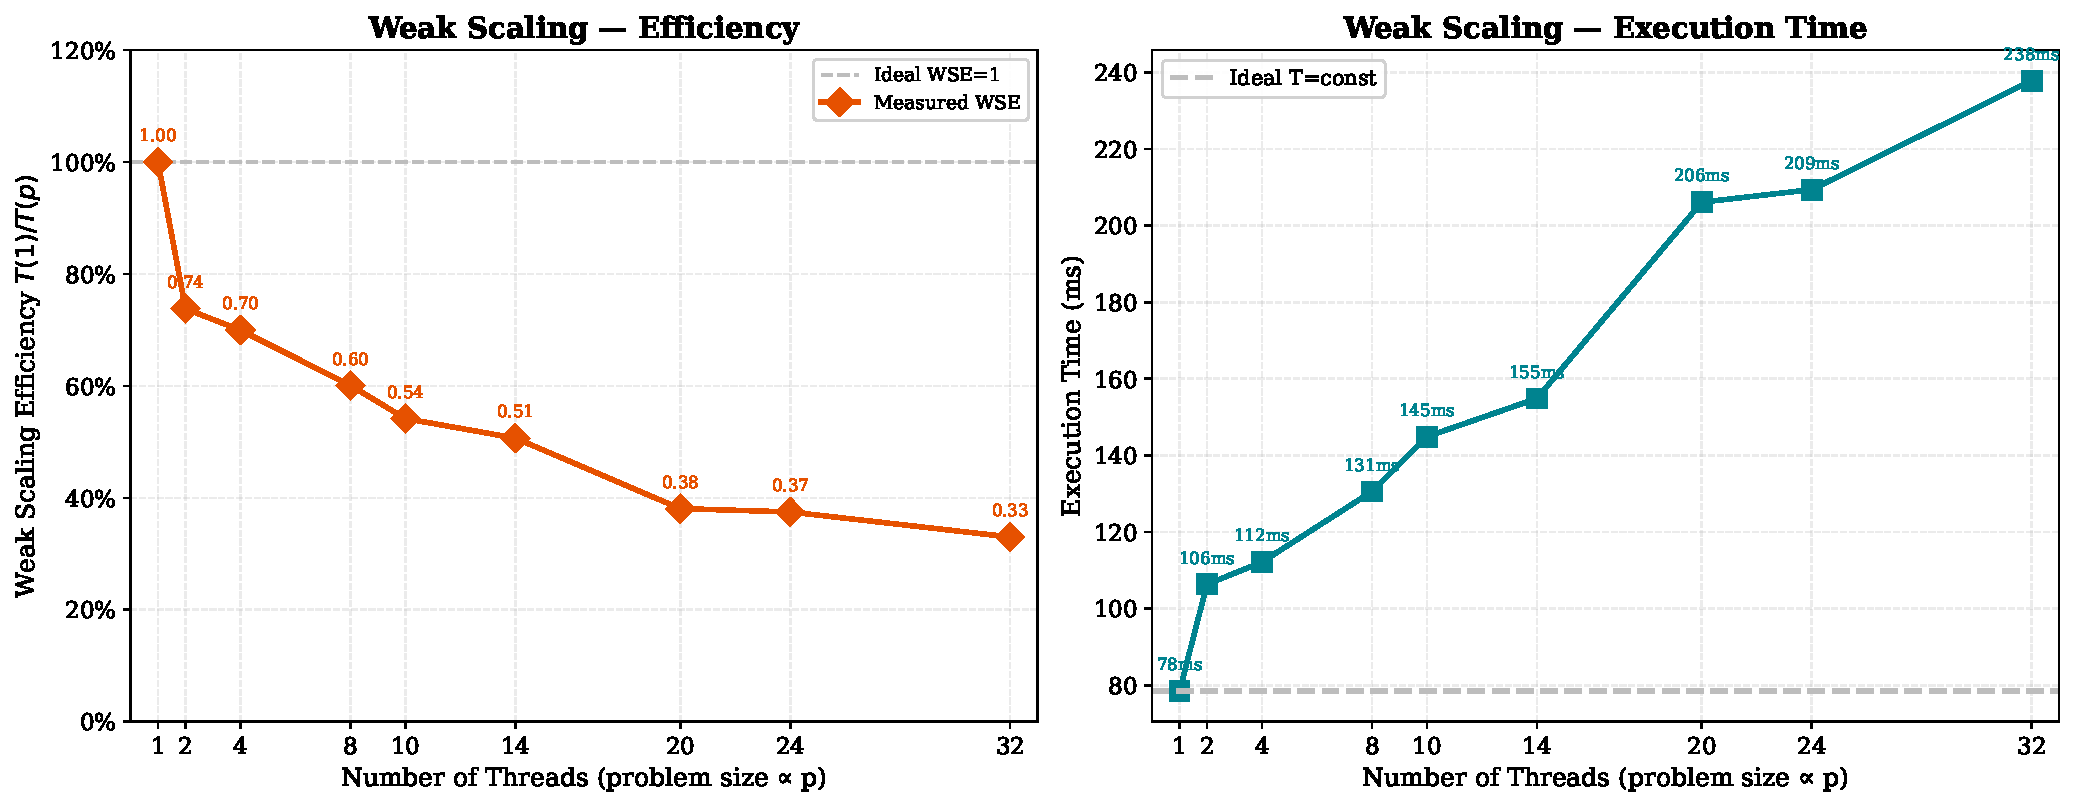
\includegraphics[width=0.85\textwidth]{../results/plots/weak_scaling.pdf}
  \caption{Weak scaling: efficiency (left) and absolute execution time (right). WSE declines monotonically; the dominant cost is scatter, whose random-write pattern saturates DRAM bandwidth as problem size grows with thread count (see \S\ref{sec:discussion}).}
  \label{fig:weak}
\end{figure*}

\subsection*{Phase Breakdown}

\begin{center}
\small
\begin{tabular}{@{}lrrrrr@{}}
\toprule
Phase & $T_\text{seq}$ & $S(14)$ & $S(20)$ & $S(24)$ & $S(32)$ \\
\midrule
Histogram R+S &  51\,ms &  2.0$\times$ &  2.4$\times$ &  3.1$\times$ &  2.7$\times$ \\
Scatter R+S   & 409\,ms &  7.8$\times$ &  9.7$\times$ & 11.3$\times$ & 13.7$\times$ \\
Join Local    & 309\,ms &  8.4$\times$ &  7.2$\times$ &  8.7$\times$ &  8.0$\times$ \\
\midrule
End-to-end    & 782\,ms &  6.7$\times$ &  7.1$\times$ &  8.0$\times$ &  8.3$\times$ \\
\bottomrule
\end{tabular}
\end{center}
{\footnotesize Individual phase times from the pipeline's internal timer. Output buffers (\texttt{out\_R}/\texttt{out\_S}) are pre-allocated before timing begins; end-to-end is the outer \texttt{Clock::now()} region and reflects only algorithmic work.}

\begin{figure}[h]
  \centering
  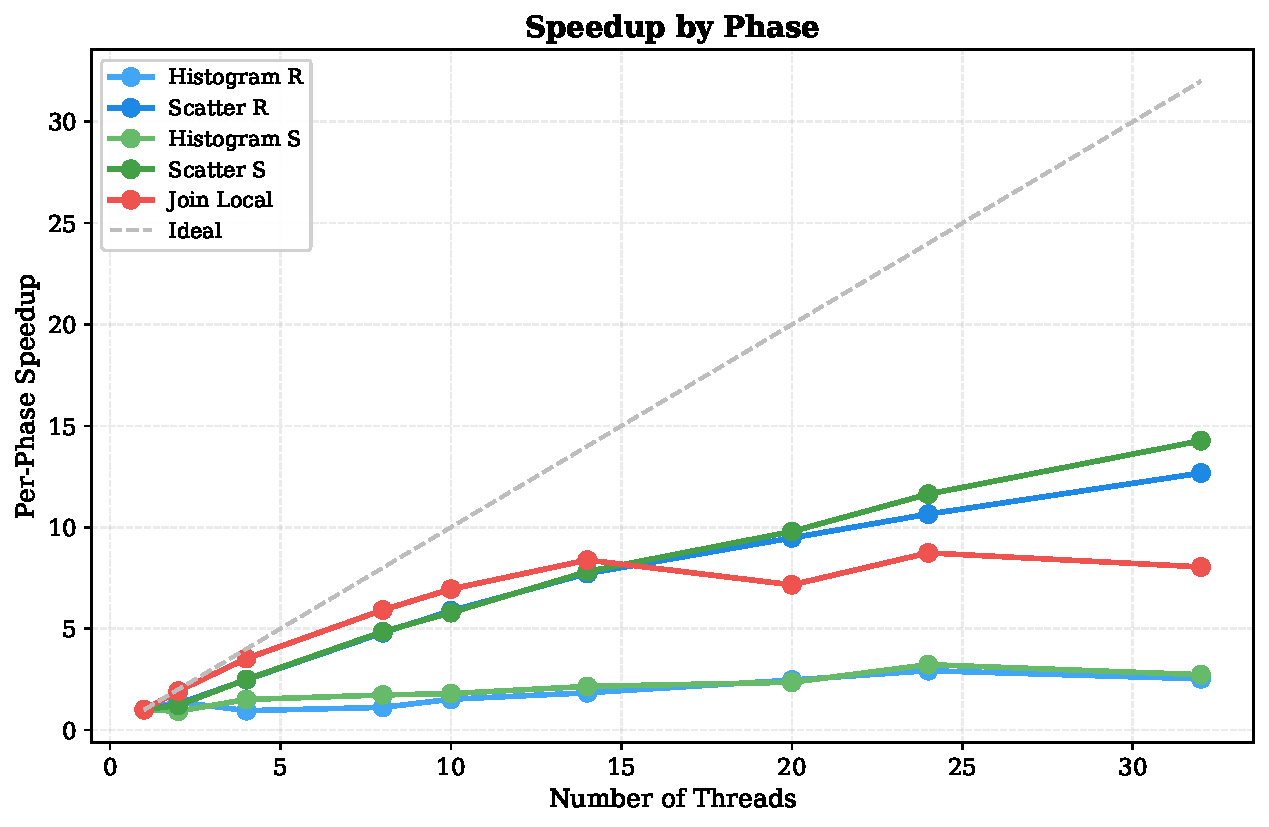
\includegraphics[width=\linewidth]{../results/plots/phase_speedup.pdf}
  \caption{Per-phase speedup across $p=1$--$32$. Join Local and Scatter scale well; Histogram is memory-bound.}
  \label{fig:phase_sp}
\end{figure}

% ===========================================================================
\section{Discussion}
\label{sec:discussion}
% ===========================================================================

\subsection*{Strong Scaling and Amdahl's Law}

Fitting Amdahl's law $S(p) = 1/(f + (1{-}f)/p)$ to the full dataset (including $p=24,32$) yields $f \approx 0.083$, giving $S_\infty = 1/f \approx 12.1\times$. Restricting the fit to physical cores ($p \leq 14$) gives $f \approx 0.092$, $S_\infty \approx 10.9\times$; the small difference ($\Delta f \approx 0.01$) confirms that the HT points do not significantly bias the estimate. The measured peak is $8.29\times$ (NR=10M, $p=32$) and $9.27\times$ (NR=20M, $p=32$) (Figures~\ref{fig:strong_speedup}--\ref{fig:strong_eff} and~\ref{fig:amdahl}). The gap between the Amdahl prediction and the measured peak is explained by memory-bandwidth saturation: as threads increase, DRAM bandwidth is the binding constraint rather than the serial fraction.

The efficiency drops from 72\% at $p=2$ to 26\% at $p=32$ (NR=10M). From $p=14$ to $p=32$, the end-to-end time improves by only $\approx 20\%$ (117\,ms $\to$ 94\,ms) despite more than doubling the thread count, making $p=14$--$20$ the practical sweet spot on this hardware. Beyond $p=16$ (HT regime), each additional logical core yields sharply diminishing returns.

\textbf{Hyper-Threading regime ($p = 20$--$32$).}
The phase breakdown reveals a counter-intuitive split at $p > 16$: scatter continues to improve (R+S combined: $9.7\times \to 13.7\times$ from $p=20$ to $p=32$) while join has a local maximum at $p=14$ ($8.4\times$), dips to $7.2\times$ at $p=20$ (HT onset), recovers to $8.7\times$ at $p=24$, then settles at $8.0\times$ at $p=32$. Scatter is memory-bandwidth-bound --- HT threads increase memory-level parallelism, so additional logical cores help. Join Local (hash-table lookups with \texttt{FlatCountMap}) is compute-bound: HT pairs share execution ports on the same physical core, so competing hash-lookup streams contend for ALU and L1/L2 resources rather than adding capacity. The net result is a moderate end-to-end gain ($7.1\times \to 8.3\times$) despite the scatter improvement. Note that with only 3 repetitions and no CPU pinning, the Join Local fluctuation ($7.2\times \to 8.7\times \to 8.0\times$ across $p=20,24,32$) should be read as a trend rather than a precise measurement; the qualitative split between a memory-bound scatter (steadily improving) and a compute-bound join (plateauing) is robust.

\begin{figure}[h]
  \centering
  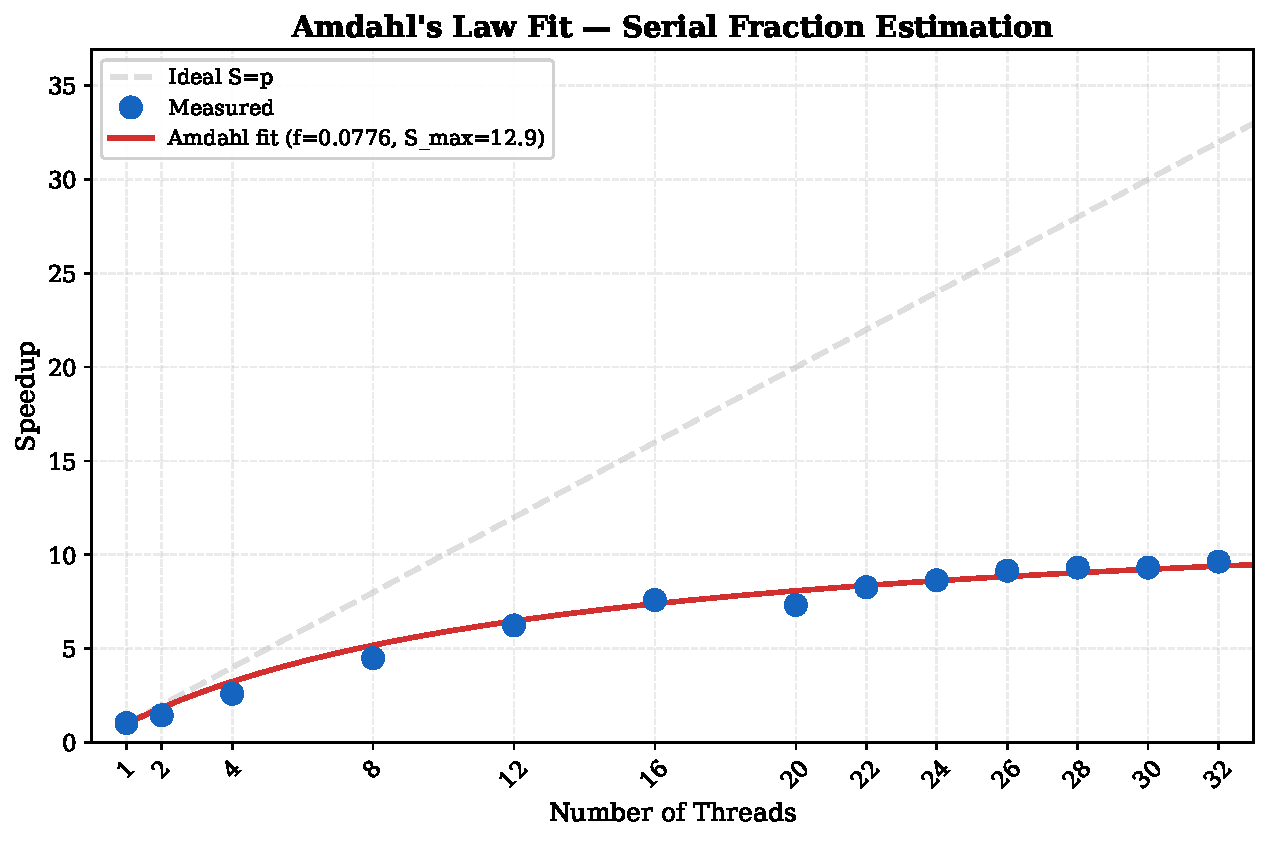
\includegraphics[width=\linewidth]{../results/plots/amdahl_fit.pdf}
  \caption{Amdahl's law fit (NR=20M). Estimated serial fraction $f \approx 0.083$; theoretical $S_\infty \approx 12.1\times$. The measured peak falls below the prediction due to memory-bandwidth saturation.}
  \label{fig:amdahl}
\end{figure}

\subsection*{Weak Scaling and WSE Interpretation}

The $p=1$ parallel binary takes $\approx 78$\,ms on NR=1M with negligible overhead from the barrier infrastructure. WSE $= T(1)/T(p)$ decreases monotonically: 0.74 at $p=2$, 0.54 at $p=10$, 0.33 at $p=32$ (Figure~\ref{fig:weak}).

The primary cause is scatter: as the problem size grows proportionally with thread count, the random-write pattern of scatter generates an increasing volume of DRAM traffic that cannot be absorbed by more cores (bandwidth is shared, not replicated). Histogram and join scale somewhat better because their access patterns benefit from per-thread private structures (thread-local histograms) or fit within the aggregate L3 capacity at low thread counts (for $p\leq 4$, each \texttt{FlatCountMap} on NR=1M/thread is $\leq 512$\,KB, well within L3). WSE drops most sharply between $p=14$ and $p=20$ ($0.51\to 0.38$, $\Delta{=}0.13$), then levels off ($p=20\to 32$: $\Delta{=}0.05$). The step coincides with the transition into the HT regime and growing NUMA penalties: with two sockets, threads on the second socket access remote memory at roughly $1.5\times$ higher latency. A structural limitation of the current implementation is that all buffers (\texttt{R}, \texttt{S}, output arrays) are allocated by the main thread on NUMA node 0; NUMA-interleaved allocation (\texttt{numactl --interleave}) would reduce remote-memory penalties and is expected to improve scalability beyond $p=8$.

\subsection*{Phase-Level Analysis}

\textbf{Histogram (2.4--3.1$\times$ at $p=20$--$32$) (Figure~\ref{fig:phase_sp}).}
Arithmetic intensity $I \approx 0.125$\,FLOP/byte places this phase firmly in the memory-bandwidth-limited region of the roofline model. Histograms account for only $\sim$7\% of sequential time, so their poor scalability affects the overall bound by $< 5\%$ (Amdahl).

\textbf{Scatter (9.7--13.7$\times$ at $p=20$--$32$).}
Scatter now dominates sequential time ($\approx 52\%$). The lock-free pre-computed-offset design eliminates all contention; speedup is limited only by DRAM write bandwidth. The continuing improvement through HT threads (Scatter improving $9.7\to 13.7\times$ from $p=20$ to $p=32$) confirms this phase benefits from increased memory-level parallelism.

\textbf{Join Local (peaks at $8.7\times$ for $p=24$, $8.0\times$ at $p=32$).}
With $P=128$ and NR=10M, each partition holds $\approx 78$K records; the \texttt{FlatCountMap} per thread occupies $\approx 4$\,MB (256K slots $\times$ 16\,B). With 20 active threads, the combined working set is $20\times 4\,\text{MB}=80$\,MB---well above the 20\,MB shared L3---so the join phase is partially DRAM-bound at $P=128$. At the optimal $P=512$, each table shrinks to $\approx 1$\,MB (64K slots), and the aggregate $\approx 20$\,MB is approximately equal to the shared L3, explaining the performance peak (see partition analysis below). The phase scales near-linearly to $p=14$ ($8.4\times$); at $p>16$ HT pairs share execution ports, causing the regression described above.

\subsection*{Partition Count Sensitivity}

With $P \in [16, 4096]$ (at $p=20$, NR=10M), execution time reaches a minimum at $P=512$--$1024$ ($\approx 86$\,ms), with a variation of $< 1.6\times$ across the full range. At $P=16$ each partition holds $\approx 625$K records and the \texttt{FlatCountMap} occupies $\approx 32$\,MB, spilling into DRAM. The optimum at $P=512$ corresponds to $\approx 20$K records/partition, with the hash table ($\approx 1$\,MB) fitting well within the shared 20\,MB L3. Beyond $P=1024$ the overhead of repeated \texttt{FlatCountMap} allocation/deallocation cycles grows: at $P=4096$ each thread performs $\approx 205$ constructor/destructor calls per join phase (vs.\ $\approx 26$ at $P=512$), increasing TLB pressure and loop overhead, raising time to 89\,ms at $P=2048$ and 94\,ms at $P=4096$. A non-monotonic bump at $P=32$ (130\,ms, slower than $P=16$) reflects a transient cache-occupancy regime between the DRAM-spill and L3-fit regions. The broad plateau around $P \in [256, 1024]$ confirms that partition count is not a critical tuning parameter (Figure~\ref{fig:part_sens}).

\begin{figure}[h]
  \centering
  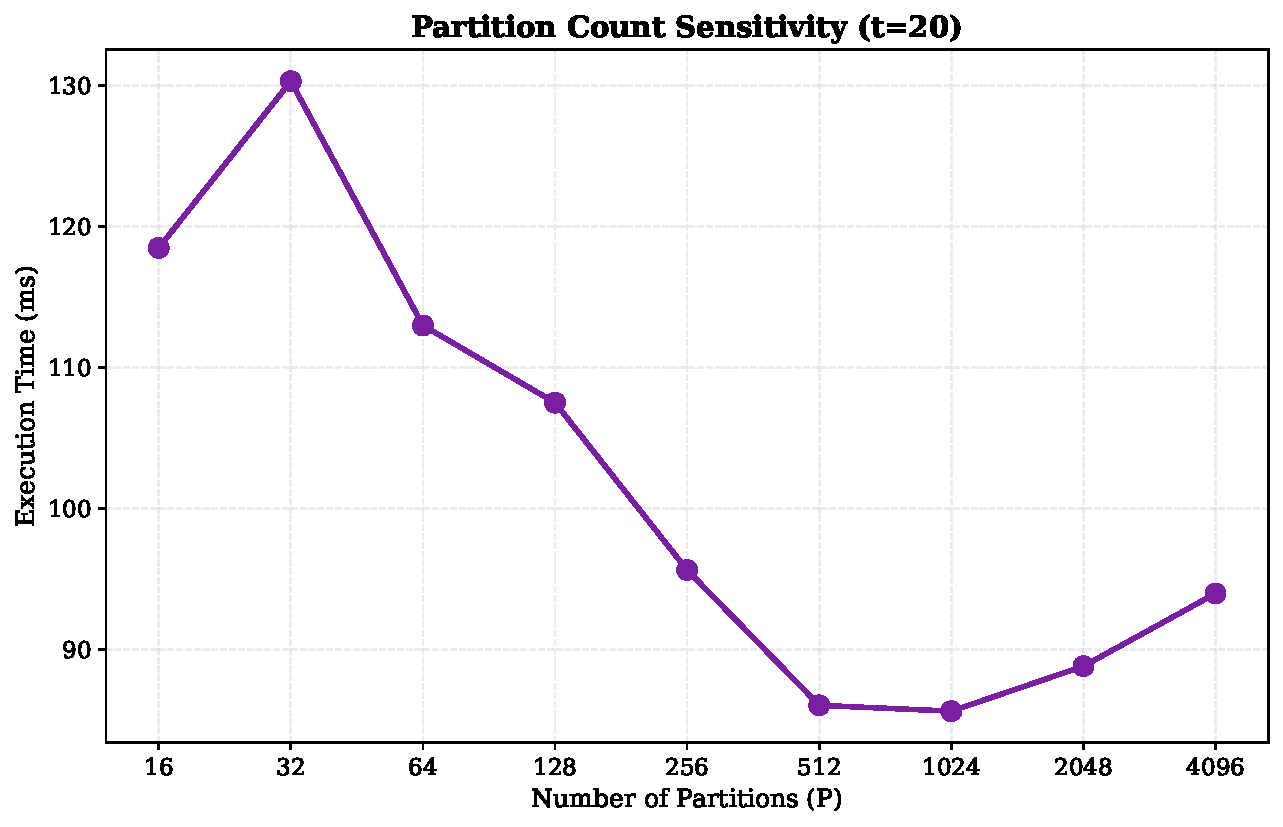
\includegraphics[width=\linewidth]{../results/plots/partition_sensitivity.pdf}
  \caption{Partition count sensitivity ($p=20$, NR=10M). Minimum at $P=512$--$1024$; non-monotonic bump at $P=32$ reflects a cache-occupancy transition.}
  \label{fig:part_sens}
\end{figure}

\subsection*{Duplicate Density}

Sequential time is essentially constant for \texttt{max\_key} $\leq 1$M ($\approx 700$--$770$\,ms): with few distinct keys the per-partition \texttt{FlatCountMap} has few occupied slots and most probes terminate immediately. At \texttt{max\_key}=10M (near-unique keys) the hash table is fully populated, increasing sequential time by $+31\%$ ($\approx 700$\,ms $\to$ 915\,ms) due to increased L3 pressure during the join phase. The parallel speedup remains stable across all duplicate densities ($\approx 6.4$--$7.5\times$ at $p=20$), confirming that partition independence is unaffected by key distribution (Figure~\ref{fig:dup}).

\begin{figure}[h]
  \centering
  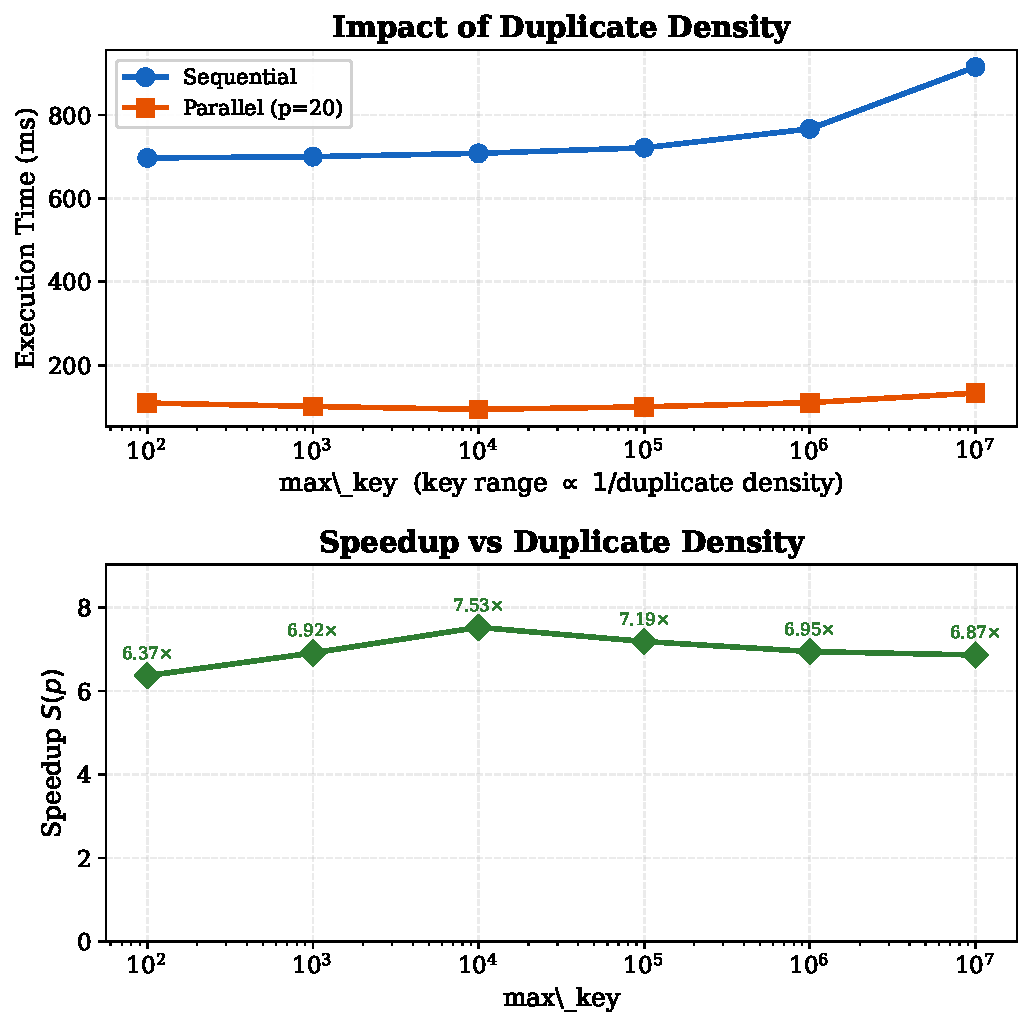
\includegraphics[width=\linewidth]{../results/plots/duplicate_density.pdf}
  \caption{Impact of duplicate density ($p=20$, NR=10M). Top: absolute execution time (seq and par). Bottom: speedup vs.\ \texttt{max\_key}. Speedup peaks at \texttt{max\_key}=10K (7.5$\times$) where keys distribute uniformly across $P=128$ partitions; at \texttt{max\_key}=100 only 100 distinct keys compete for 128 partitions, causing load imbalance and lower speedup (6.4$\times$).}
  \label{fig:dup}
\end{figure}

\end{document}
